\section{Closing Thoughts}

\begin{frame}{Closing Thoughts: Challenges and Reflection}
\begin{columns}
\begin{column}{0.6\textwidth}
\begin{itemize}
\item data management
\begin{itemize}
	\item save data trial-wise instead of batch-wise
    \item export to standard format
\end{itemize}
\item Jupyter notebooks
\begin{itemize}
	\item write frequently used analysis functions into package
\end{itemize}
\item compute time
\begin{itemize}
	\item seek grant funding for more stable compute environment
\end{itemize}
\end{itemize}
\end{column}
\begin{column}{0.4\textwidth}
\begin{center}
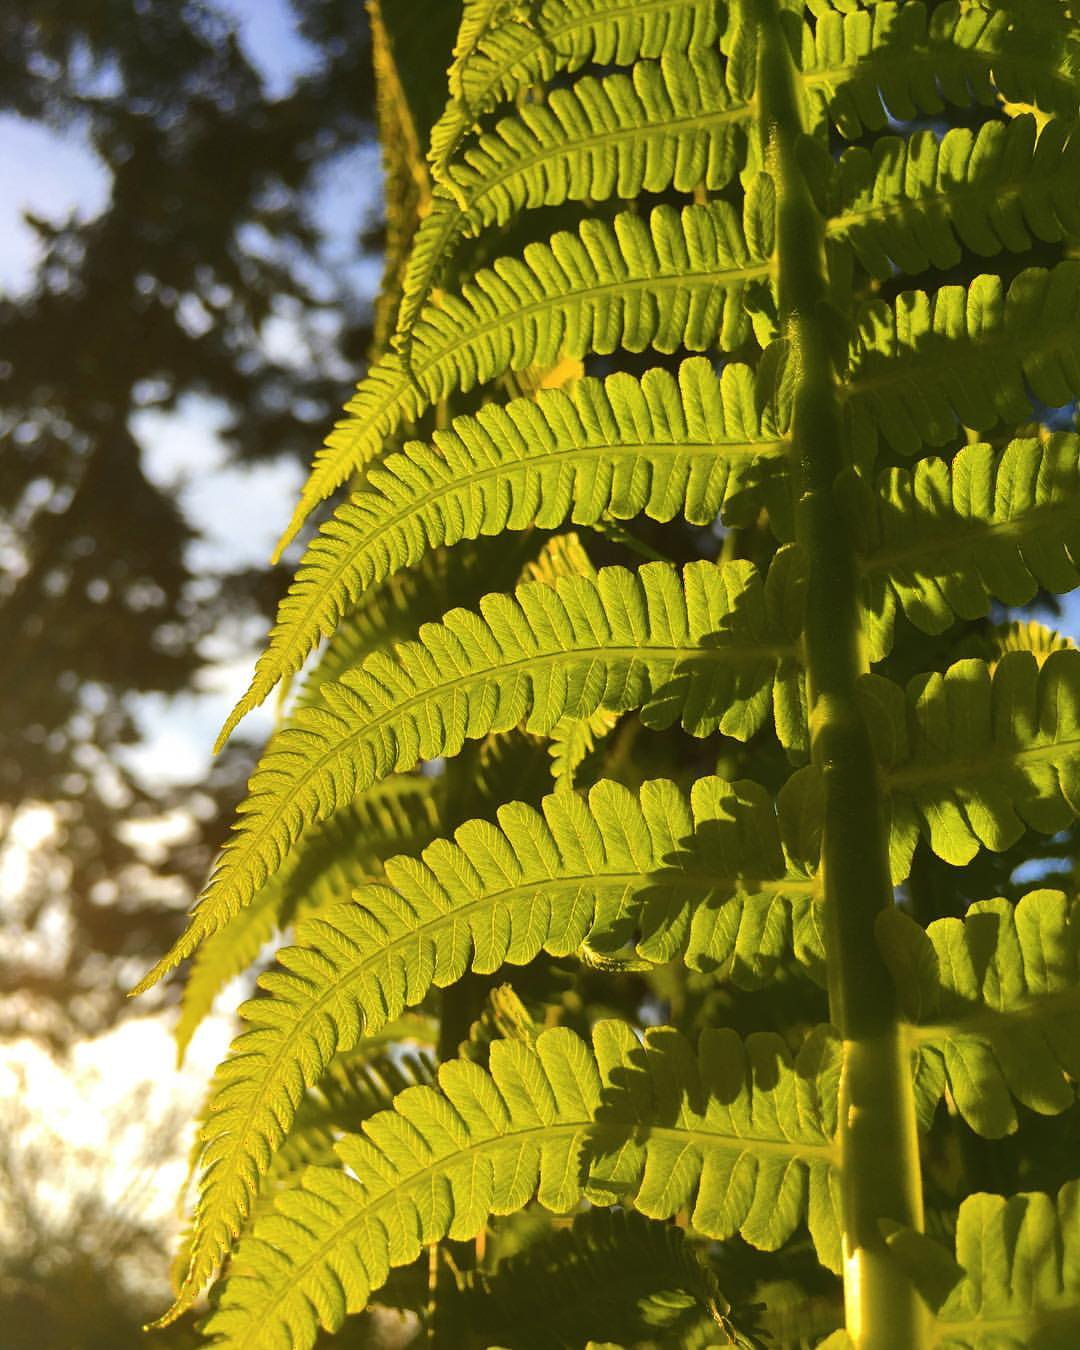
\includegraphics[width=\textwidth,trim={0cm 0 6cm 0},clip]{img/sunset_fern}
\end{center}
\end{column}
\end{columns}
\end{frame}

\begin{frame}{Closing Thoughts: Next Steps}
\begin{columns}
\begin{column}{0.6\textwidth}
\begin{itemize}
\item more directly biologically-inspired model
\item attempt to demonstrate situation where search with plasticity outperforms search without
\end{itemize}
\end{column}
\begin{column}{0.4\textwidth}
\begin{center}
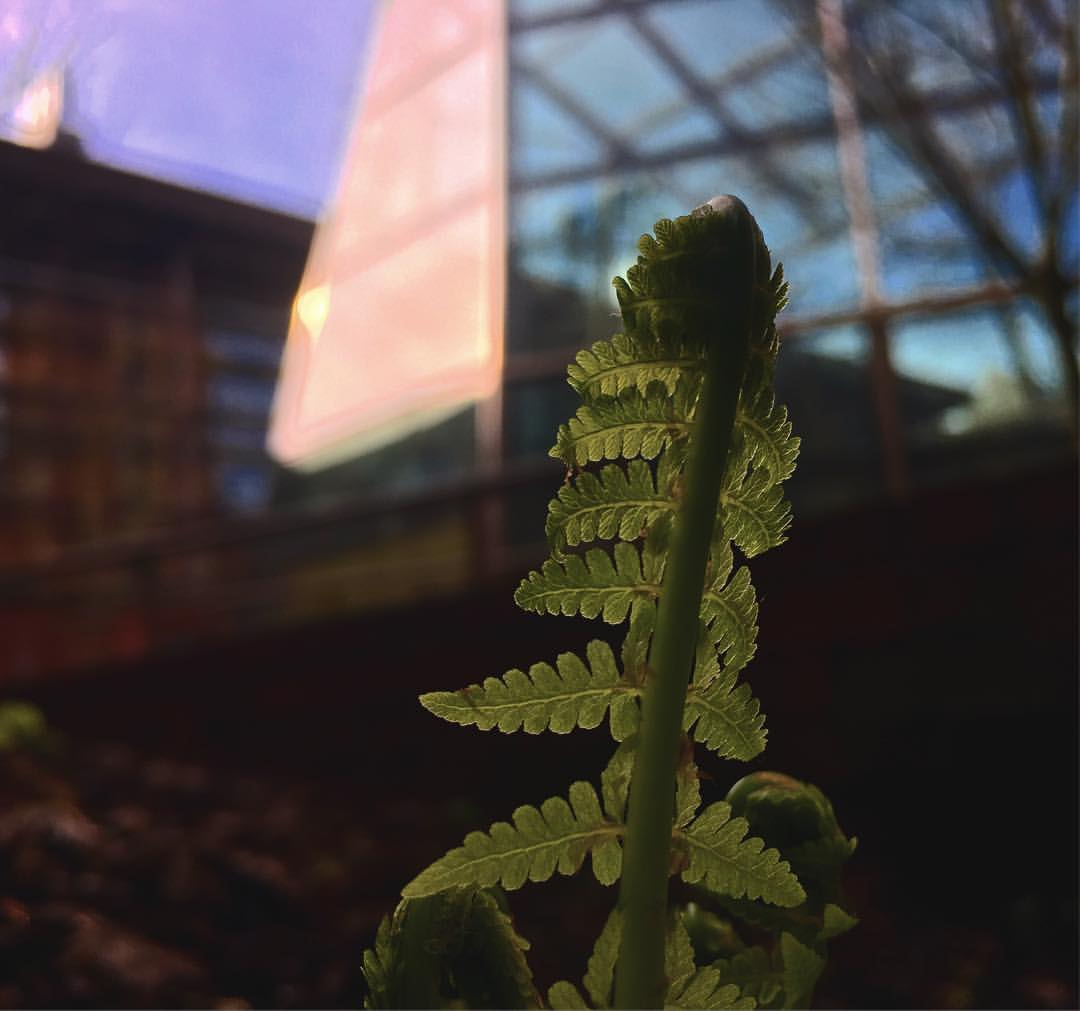
\includegraphics[width=\textwidth,trim={7cm 0 8cm 0},clip]{img/oppfern}
\end{center}
\end{column}
\end{columns}
\end{frame}

% \begin{frame}{Closing Thoughts: Scientific Questions}
% \begin{columns}
% \begin{column}{0.6\textwidth}
% \begin{itemize}
% \item at what level of abstraction can the power of biological evolution be harnessed in a computational model?
% \item what are the fundamental mechanisms at play in evolution?
% \end{itemize}
% \end{column}
% \begin{column}{0.4\textwidth}
% \begin{center}
% 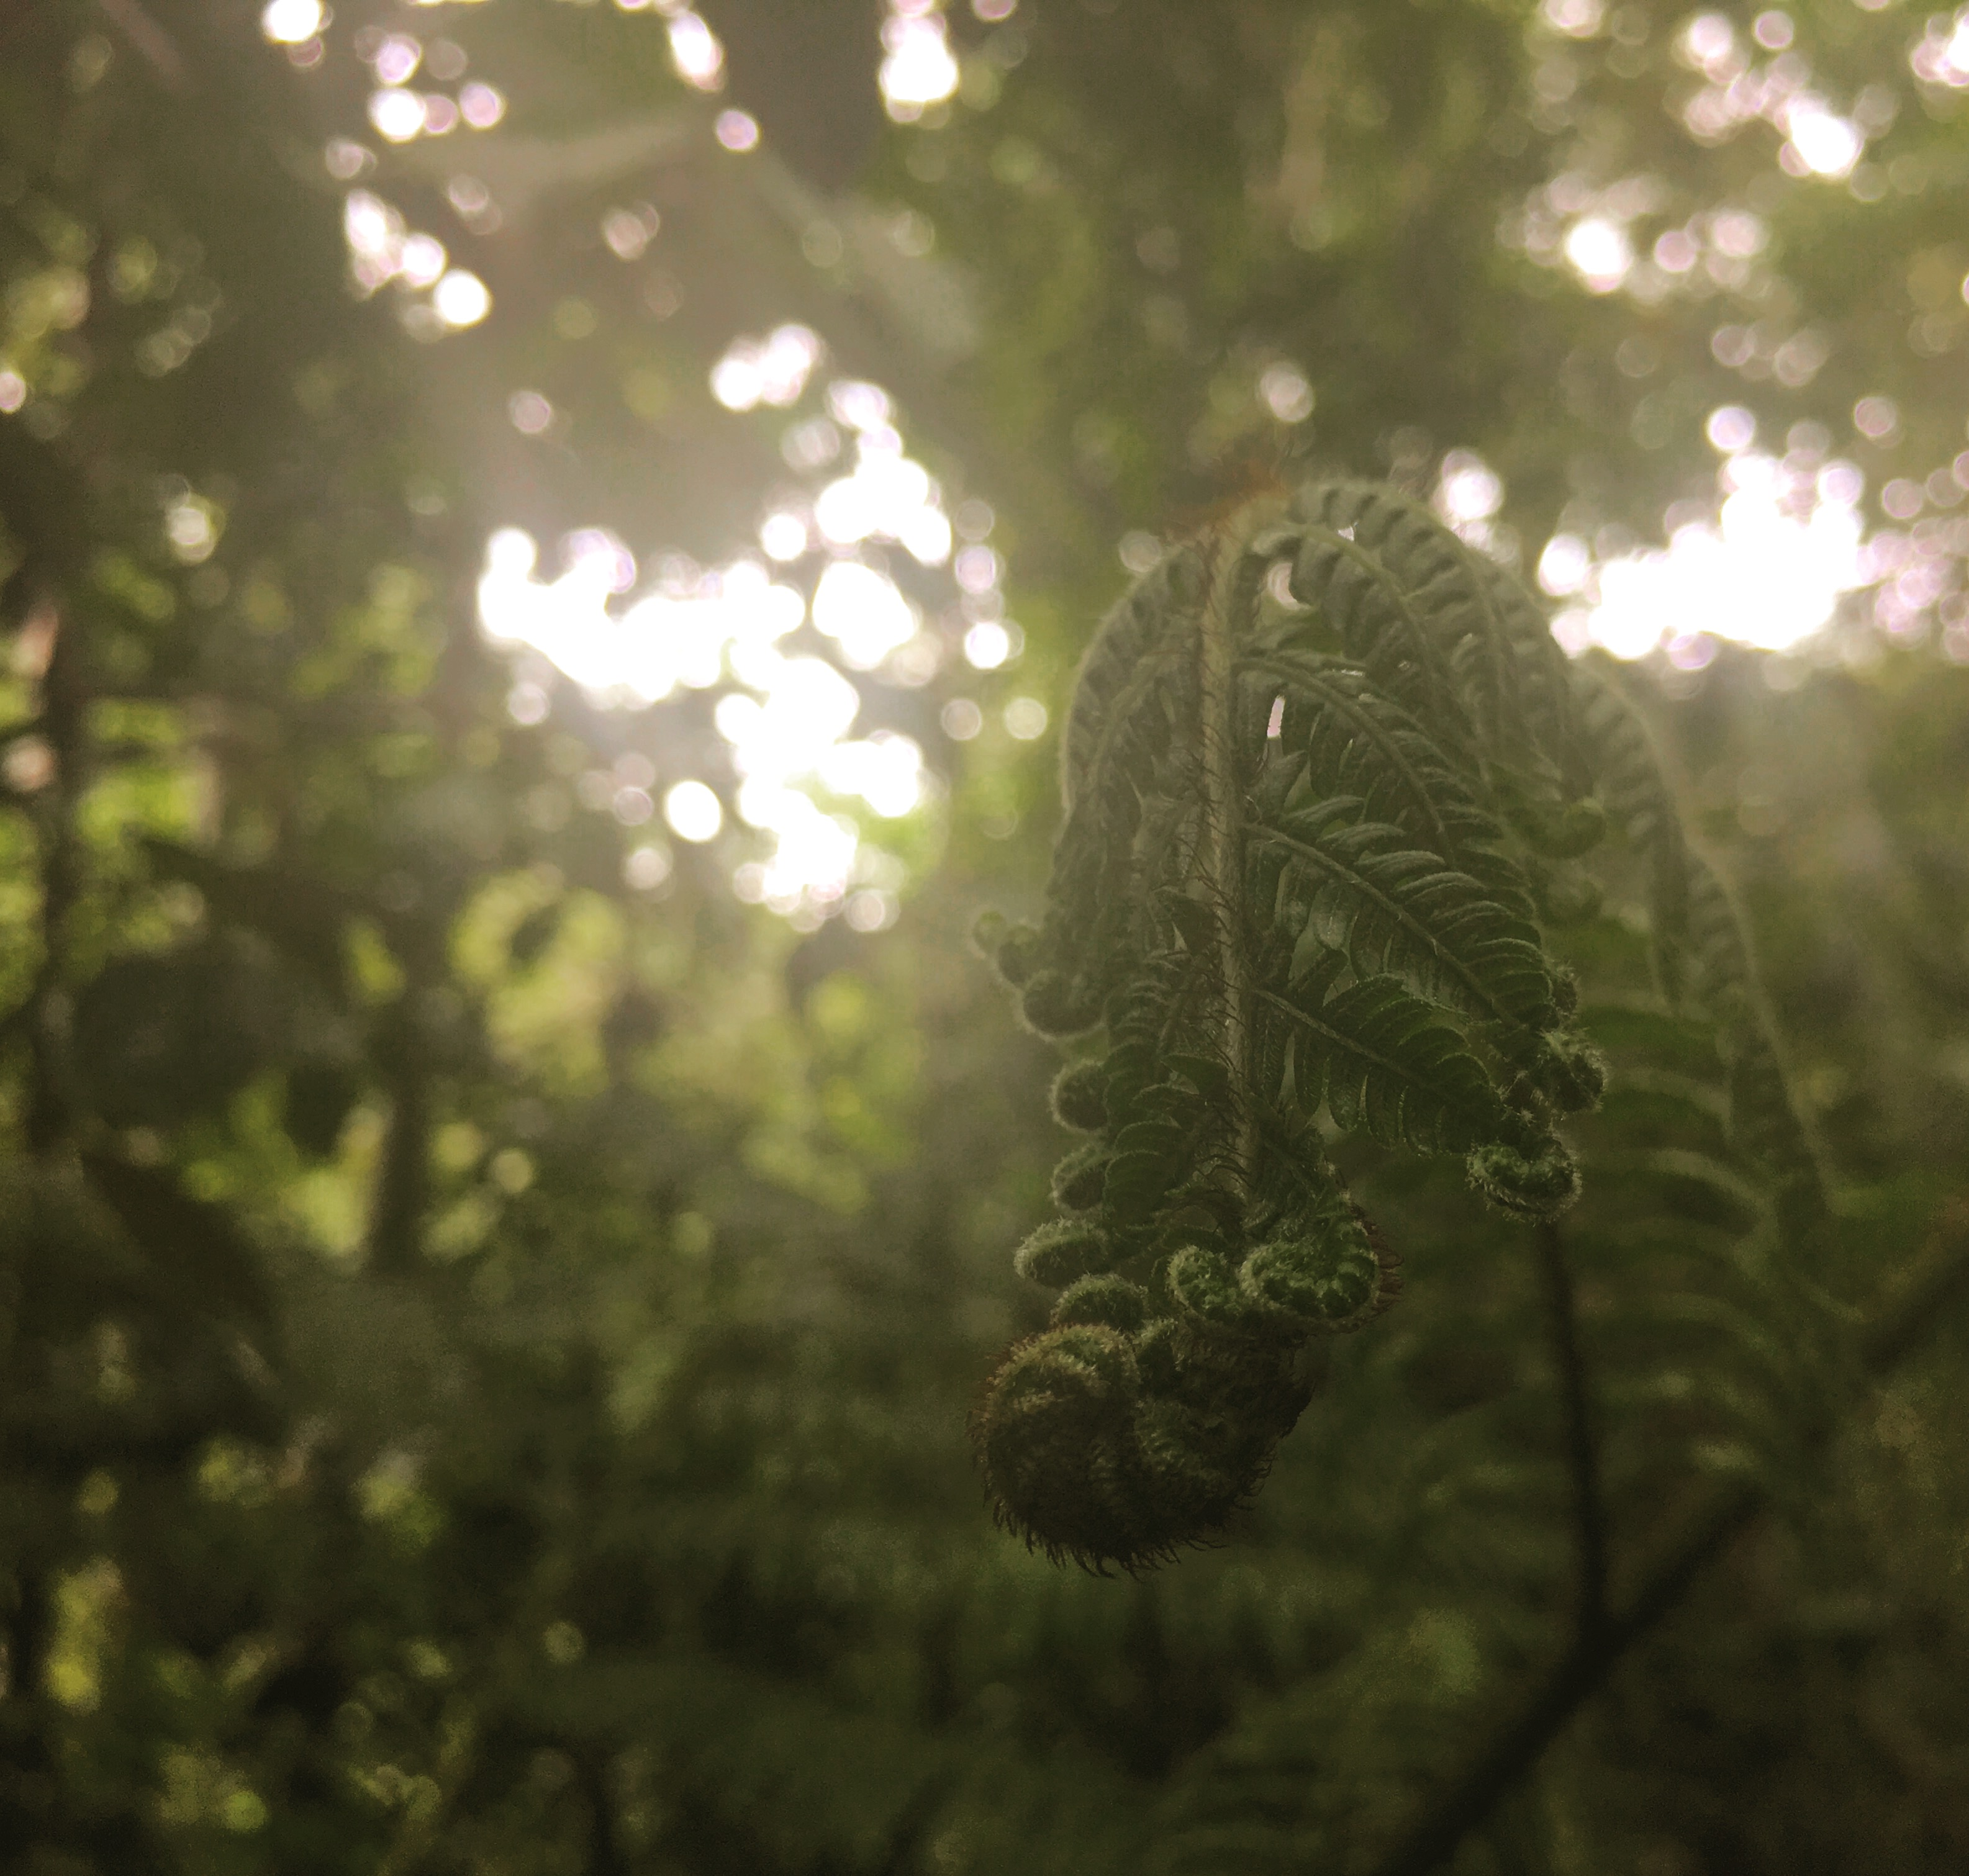
\includegraphics[width=\textwidth,trim={18cm 0 27cm 0},clip]{img/tropical_fern}
% \end{center}
% \end{column}
% \end{columns}
% \end{frame}

% \begin{frame}{Closing Thoughts: Scientific Questions}
% \begin{columns}
% \begin{column}{0.6\textwidth}
% \begin{itemize}
% \item evolutionary biology provides continuing inspiration for new techniques in evolutionary computing
% \item evolutionary models move theory evaluation from a qualitative endeavor towards a quantitative endeavor
% \end{itemize}
% \end{column}
% \begin{column}{0.4\textwidth}
% \begin{center}
% 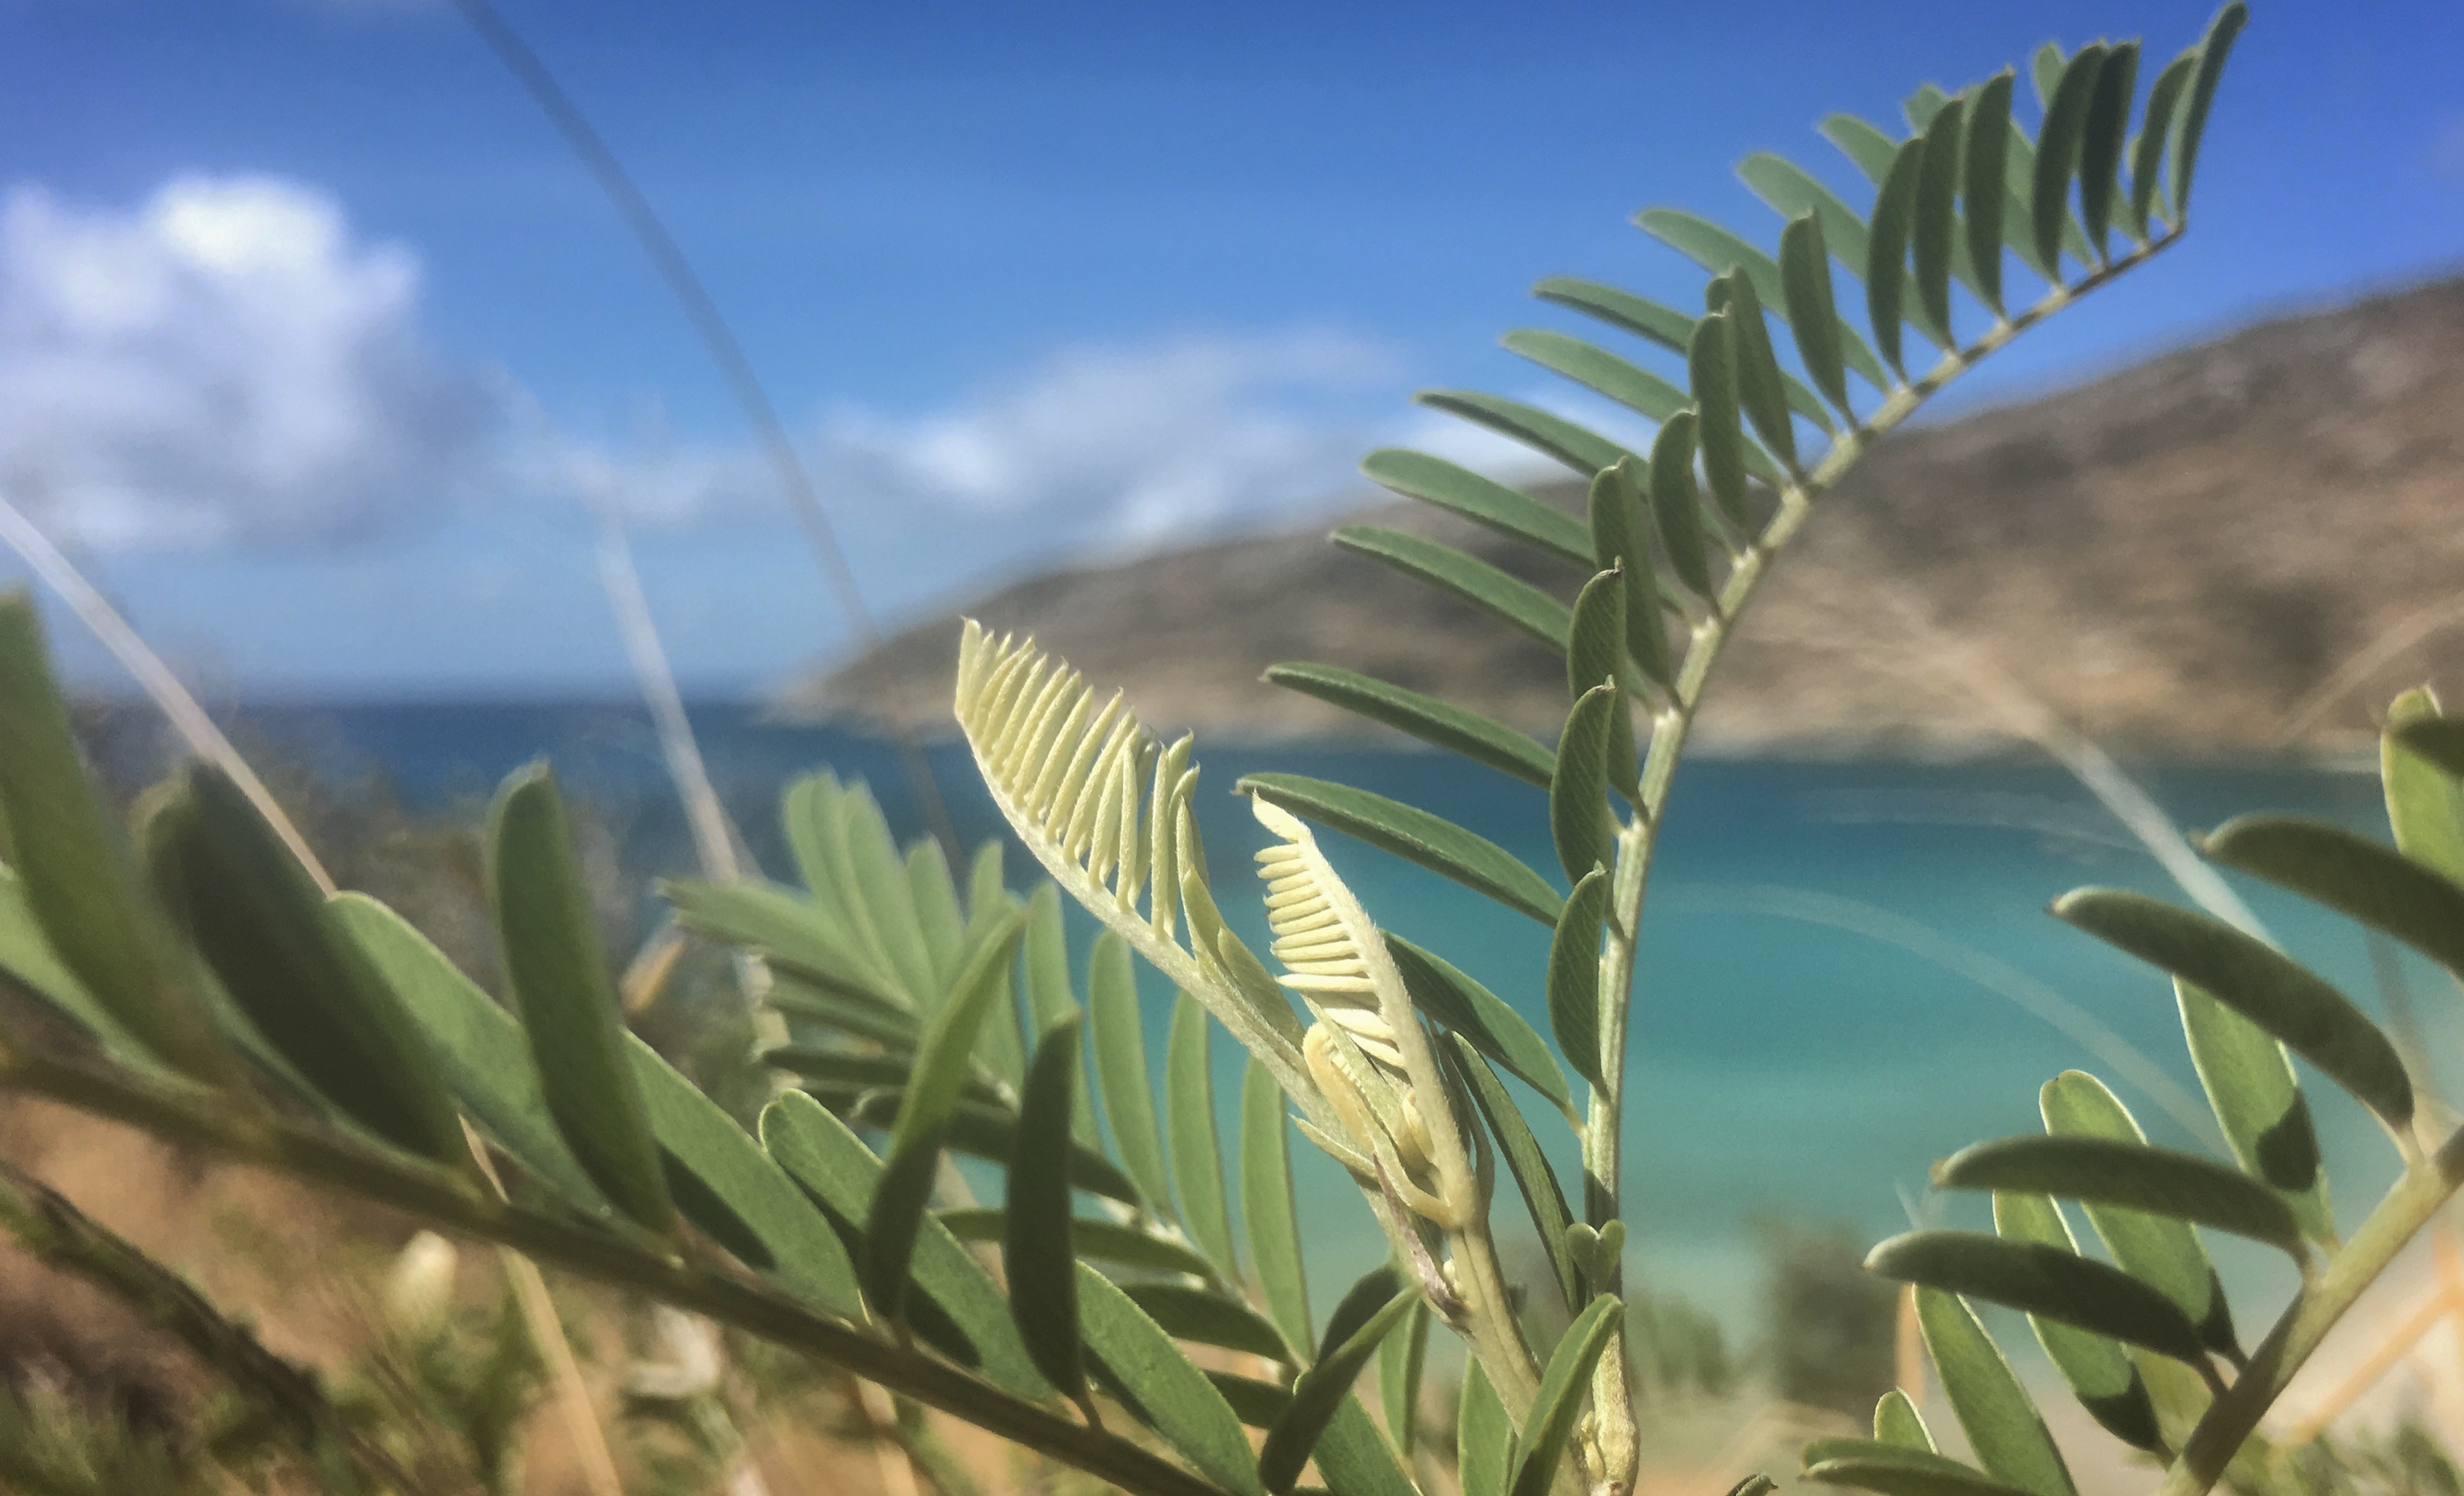
\includegraphics[width=\textwidth,trim={43cm 0 47cm 0},clip]{img/island_fern}
% \end{center}
% \end{column}
% \end{columns}
% \end{frame}

% \begin{frame}{Scientific Questions}
% \begin{displayquote}
% ``Many evolutionary biologists do not see a need to connect somatic adaptability to the generation of variation, and some see a need to keep them separate. For them, it is sufficient to say that random mutation is required and that the phenotypic variation arises haphazardly from it as random damage; the organism's current phenotype does not matter for the variation produced, and the output of variation is nearly random \cite[p 219]{Kirschner2005TheDilemma}.''
% \end{displayquote}
% \end{frame}